\documentclass{ximera}

%\usepackage{todonotes}

\newcommand{\todo}{}

\usepackage{tkz-euclide}
\tikzset{>=stealth} %% cool arrow head
\tikzset{shorten <>/.style={ shorten >=#1, shorten <=#1 } } %% allows shorter vectors

\usepackage{tkz-tab}  %% sign charts
\usetikzlibrary{decorations.pathreplacing} 

\usetikzlibrary{backgrounds} %% for boxes around graphs
\usetikzlibrary{shapes,positioning}  %% Clouds and stars
\usetikzlibrary{matrix} %% for matrix
\usepgfplotslibrary{polar} %% for polar plots
\usetkzobj{all}
\usepackage[makeroom]{cancel} %% for strike outs
%\usepackage{mathtools} %% for pretty underbrace % Breaks Ximera
\usepackage{multicol}

\usepackage{polynom}



\usepackage[many]{tcolorbox}  %% for titled boxes
\newtcolorbox{xbox}[1]{%
    tikznode boxed title,
    enhanced,
    arc=0mm,
    interior style={white},
    attach boxed title to top center= {yshift=-\tcboxedtitleheight/2},
    fonttitle=\bfseries,
    colbacktitle=white,coltitle=black,
    boxed title style={size=normal,colframe=white,boxrule=0pt},
    title={#1}}


\usepackage{array}
\setlength{\extrarowheight}{+.1cm}   
\newdimen\digitwidth
\settowidth\digitwidth{9}
\def\divrule#1#2{
\noalign{\moveright#1\digitwidth
\vbox{\hrule width#2\digitwidth}}}





\newcommand{\RR}{\mathbb R}
\newcommand{\R}{\mathbb R}
\newcommand{\N}{\mathbb N}
\newcommand{\Z}{\mathbb Z}

%\renewcommand{\d}{\,d\!}
\renewcommand{\d}{\mathop{}\!d}
\newcommand{\dd}[2][]{\frac{\d #1}{\d #2}}
\newcommand{\pp}[2][]{\frac{\partial #1}{\partial #2}}
\renewcommand{\l}{\ell}
\newcommand{\ddx}{\frac{d}{\d x}}
\newcommand{\ddt}{\frac{d}{\d t}}

\newcommand{\zeroOverZero}{\ensuremath{\boldsymbol{\tfrac{0}{0}}}}
\newcommand{\inftyOverInfty}{\ensuremath{\boldsymbol{\tfrac{\infty}{\infty}}}}
\newcommand{\zeroOverInfty}{\ensuremath{\boldsymbol{\tfrac{0}{\infty}}}}
\newcommand{\zeroTimesInfty}{\ensuremath{\small\boldsymbol{0\cdot \infty}}}
\newcommand{\inftyMinusInfty}{\ensuremath{\small\boldsymbol{\infty - \infty}}}
\newcommand{\oneToInfty}{\ensuremath{\boldsymbol{1^\infty}}}
\newcommand{\zeroToZero}{\ensuremath{\boldsymbol{0^0}}}
\newcommand{\inftyToZero}{\ensuremath{\boldsymbol{\infty^0}}}



\newcommand{\numOverZero}{\ensuremath{\boldsymbol{\tfrac{\#}{0}}}}
\newcommand{\dfn}{\textbf}
%\newcommand{\unit}{\,\mathrm}
\newcommand{\unit}{\mathop{}\!\mathrm}
\newcommand{\eval}[1]{\bigg[ #1 \bigg]}
\newcommand{\seq}[1]{\left( #1 \right)}
\renewcommand{\epsilon}{\varepsilon}
\renewcommand{\iff}{\Leftrightarrow}

\DeclareMathOperator{\arccot}{arccot}
\DeclareMathOperator{\arcsec}{arcsec}
\DeclareMathOperator{\arccsc}{arccsc}
\DeclareMathOperator{\si}{Si}
\DeclareMathOperator{\proj}{proj}
\DeclareMathOperator{\scal}{scal}


\newcommand{\tightoverset}[2]{% for arrow vec
  \mathop{#2}\limits^{\vbox to -.5ex{\kern-0.75ex\hbox{$#1$}\vss}}}
\newcommand{\arrowvec}[1]{\tightoverset{\scriptstyle\rightharpoonup}{#1}}
\renewcommand{\vec}{\mathbf}
\newcommand{\veci}{\vec{i}}
\newcommand{\vecj}{\vec{j}}
\newcommand{\veck}{\vec{k}}
\newcommand{\vecl}{\boldsymbol{\l}}

\newcommand{\dotp}{\bullet}
\newcommand{\cross}{\boldsymbol\times}
\newcommand{\grad}{\boldsymbol\nabla}
\newcommand{\divergence}{\grad\dotp}
\newcommand{\curl}{\grad\cross}
%\DeclareMathOperator{\divergence}{divergence}
%\DeclareMathOperator{\curl}[1]{\grad\cross #1}


\colorlet{textColor}{black} 
\colorlet{background}{white}
\colorlet{penColor}{blue!50!black} % Color of a curve in a plot
\colorlet{penColor2}{red!50!black}% Color of a curve in a plot
\colorlet{penColor3}{red!50!blue} % Color of a curve in a plot
\colorlet{penColor4}{green!50!black} % Color of a curve in a plot
\colorlet{penColor5}{orange!80!black} % Color of a curve in a plot
\colorlet{fill1}{penColor!20} % Color of fill in a plot
\colorlet{fill2}{penColor2!20} % Color of fill in a plot
\colorlet{fillp}{fill1} % Color of positive area
\colorlet{filln}{penColor2!20} % Color of negative area
\colorlet{fill3}{penColor3!20} % Fill
\colorlet{fill4}{penColor4!20} % Fill
\colorlet{fill5}{penColor5!20} % Fill
\colorlet{gridColor}{gray!50} % Color of grid in a plot

\newcommand{\surfaceColor}{violet}
\newcommand{\surfaceColorTwo}{redyellow}
\newcommand{\sliceColor}{greenyellow}




\pgfmathdeclarefunction{gauss}{2}{% gives gaussian
  \pgfmathparse{1/(#2*sqrt(2*pi))*exp(-((x-#1)^2)/(2*#2^2))}%
}


%%%%%%%%%%%%%
%% Vectors
%%%%%%%%%%%%%

%% Simple horiz vectors
\renewcommand{\vector}[1]{\left\langle #1\right\rangle}


%% %% Complex Horiz Vectors with angle brackets
%% \makeatletter
%% \renewcommand{\vector}[2][ , ]{\left\langle%
%%   \def\nextitem{\def\nextitem{#1}}%
%%   \@for \el:=#2\do{\nextitem\el}\right\rangle%
%% }
%% \makeatother

%% %% Vertical Vectors
%% \def\vector#1{\begin{bmatrix}\vecListA#1,,\end{bmatrix}}
%% \def\vecListA#1,{\if,#1,\else #1\cr \expandafter \vecListA \fi}

%%%%%%%%%%%%%
%% End of vectors
%%%%%%%%%%%%%

%\newcommand{\fullwidth}{}
%\newcommand{\normalwidth}{}



%% makes a snazzy t-chart for evaluating functions
%\newenvironment{tchart}{\rowcolors{2}{}{background!90!textColor}\array}{\endarray}

%%This is to help with formatting on future title pages.
\newenvironment{sectionOutcomes}{}{} 



%% Flowchart stuff
%\tikzstyle{startstop} = [rectangle, rounded corners, minimum width=3cm, minimum height=1cm,text centered, draw=black]
%\tikzstyle{question} = [rectangle, minimum width=3cm, minimum height=1cm, text centered, draw=black]
%\tikzstyle{decision} = [trapezium, trapezium left angle=70, trapezium right angle=110, minimum width=3cm, minimum height=1cm, text centered, draw=black]
%\tikzstyle{question} = [rectangle, rounded corners, minimum width=3cm, minimum height=1cm,text centered, draw=black]
%\tikzstyle{process} = [rectangle, minimum width=3cm, minimum height=1cm, text centered, draw=black]
%\tikzstyle{decision} = [trapezium, trapezium left angle=70, trapezium right angle=110, minimum width=3cm, minimum height=1cm, text centered, draw=black]


\title[Dig-In:]{Horizontal asymptotes}

\outcome{Find horizontal asymptotes using limits.}
\outcome{Recognize that a curve can cross a horizontal asymptote.}
\outcome{Calculate the limit as $x$ approaches $\pm \infty$ of common functions algebraically.}
\outcome{Find the limit as $x$ approaches $\pm \infty$ from a graph.}
\outcome{Define a horizontal asymptote.}
\outcome{Compute limits at infinity of famous functions.}
\outcome{Identify horizontal asymptotes by looking at a graph.}

\begin{document}
\begin{abstract}
We explore functions that behave like horizontal lines as the input
grows without bound.
\end{abstract}
\maketitle



Let's start with an example:
\begin{example}
	Consider the function:
	\[ g(x) = \frac{1}{x} \]
	with the table below
	\[ \begin{array}{c|c}
		x       & g(x)=\frac{1}{x} \\\hline
		10      & \answer[given]{0.1} \\ 
		100     & \answer[given]{0.01} \\
		1000    & \answer[given]{0.001} \\
		10000   & \answer[given]{0.0001} \\
		100000  & \answer[given]{0.00001}\\
		1000000 & \answer[given]{0.000001}
	\end{array} \]

	What does the table tell us about $g(x)$ as $x$ grows bigger and bigger?
	\begin{explanation}
		As $x$ grows bigger and bigger, it seems that $g(x)$ approaches $0$. It seems that we should write
		\[ \lim_{x\to \infty}\frac{1}{x}=0 \]
	\end{explanation}
\end{example}

\begin{example}
  Now consider a different function:
  \[
  f(x) = \frac{6x-9}{x-1}
  \]
  \begin{image}
    \begin{tikzpicture}
      \begin{axis}[
          domain=1:4,
          ymax=20,
          ymin=-10,
          samples=100,
          axis lines =middle, xlabel=$x$, ylabel=$y$,
          every axis y label/.style={at=(current axis.above origin),anchor=south},
          every axis x label/.style={at=(current axis.right of origin),anchor=west}
        ]
	\addplot [very thick, penColor, smooth, domain=(0:.9)] {(6*x-9)/(x-1)};
        \addplot [very thick, penColor, smooth, domain=(1.1:3)] {(6*x-9)/(x-1)};
        \addplot [textColor, dashed] plot coordinates {(1,-10) (1,20)};
        \addplot [textColor, dashed] plot coordinates {(0,6) (3,6)};
      \end{axis}
    \end{tikzpicture}

  \end{image}

  Fill in the table below, rounding to $5$ decimal places.
  \[
  \begin{array}{c|c}
    x      & f(x)=\frac{6x-9}{x-1} \\ \hline
    10     & \answer[given]{5.66667}\\
    100    & \answer[given]{5.96970}\\
    1000   & \answer[given]{5.99700}\\
    10000  & \answer[given]{5.99970}\\
    100000 & \answer[given]{5.99997}\\
  \end{array}
  \]
  What does the table tell us about $f(x)$ as $x$ grows bigger and bigger?
  \begin{explanation}
    As $x$ grows bigger and bigger, it seems like $f(x)$ approaches $6$.
    It seems that we should write
    \[
    \lim_{x\to \infty}\frac{6x-9}{x-1}=6 
    \]
  \end{explanation}
\end{example}

\begin{definition}\label{def:limitAtInfty}\index{limit!at infinity}
If $f(x)$ becomes arbitrarily close to a specific value $L$ by making
$x$ sufficiently large, we write
\[
\lim_{x\to \infty} f(x) = L
\]
and we say, the \dfn{limit at infinity} of $f(x)$ is $L$.  

If $f(x)$ becomes arbitrarily close to a specific value $L$ by making
$x$ sufficiently large and negative, we write
\[
\lim_{x\to -\infty} f(x) = L
\]
and we say, the \dfn{limit at negative infinity} of $f(x)$ is $L$.  
\end{definition}

\begin{example}  Compute the limit.
\[
\lim_{x\to\infty} \frac{6x-9}{x-1}.
\]
We will confirm what we guessed earlier by computing the limit at infinity.\\
 We can assume that all the Limit Laws also apply to limits at infinity.
\begin{explanation}
Write
\begin{align*}
\lim_{x\to\infty}\frac{6x-9}{x-1} &= \lim_{x\to\infty}\frac{6x-9}{x-1}\cdot \frac{1/x}{1/x}\\
&=\lim_{x\to\infty}\frac{\frac{6x}{x} - \frac{9}{x}}{\frac{x}{x} - \frac{1}{x}}\\
&=\frac{\lim_{x\to\infty}\Bigl(6- \frac{9}{x}\Bigr)}{\lim_{x\to\infty}\Bigl(1- \frac{1}{x}\Bigr)}\\
&=\frac{6-9\lim_{x\to\infty}  \frac{1}{x}}{1-\lim_{x\to\infty} \frac{1}{x}}\\
&=\frac{6-9(0)}{1-0}\\
&=  \frac{6}{1}\\
&= 6.
\end{align*}
\end{explanation}
\end{example}

Sometimes one must be careful, consider this example.

\begin{example}

\[
\lim_{x\to -\infty} \frac{x^3+1}{\sqrt{x^6+5}}
\]
\begin{explanation}
In this case we multiply the numerator and denominator by $-1/x^3$,
which is a positive number as since $x\to -\infty$, $x^3$ is a negative
number.
\begin{align*}
\lim_{x\to -\infty} \frac{x^3+1}{\sqrt{x^6+5}} &= \lim_{x\to -\infty} \frac{x^3+1}{\sqrt{x^6+5}} \cdot \frac{-1/x^3}{-1/x^3}\\
&= \lim_{x\to -\infty} \frac{-1-1/x^3}{\sqrt{x^6/x^6+5/x^6}}\\
&= \lim_{x\to -\infty} \frac{-1-1/x^3}{\sqrt{1+5/x^6}}\\
&= \frac{ \lim_{x\to -\infty}\Bigl(-1-1/x^3\Bigr)}{\lim_{x\to -\infty}\sqrt{1+5/x^6}}\\
&= \frac{ -1-\lim_{x\to -\infty}(1/x)^3}{\sqrt{\lim_{x\to -\infty}\Bigl(1+5/x^6\Bigr)}}\\
&= \frac{ -1-(\lim_{x\to -\infty}1/x)^3}{\sqrt{1+5(\lim_{x\to -\infty}1/x)^6}}\\
&= \frac{ -1-(0)^3}{\sqrt{1+5(0)^6}}\\
&= \frac{ -1-0}{\sqrt{1+0}}\\
&= -1.
\end{align*}
\end{explanation}
\end{example}

Note, since
\[
\lim_{x\to \infty} f(x) = \lim_{x\to 0^+} f\left(\frac{1}{x}\right)
\]
and
\[
\lim_{x\to -\infty} f(x) = \lim_{x\to 0^-} f\left(\frac{1}{x}\right)
\]
we can also apply the Squeeze Theorem when taking limits at infinity.
Here is an example of a limit at infinity that uses the Squeeze
Theorem, and shows that functions can, in fact, cross their horizontal
asymptotes.


\begin{example}
Compute:
\[
\lim_{x\to \infty} \frac{\sin(7x)+4x}{x}
\]
\begin{image}
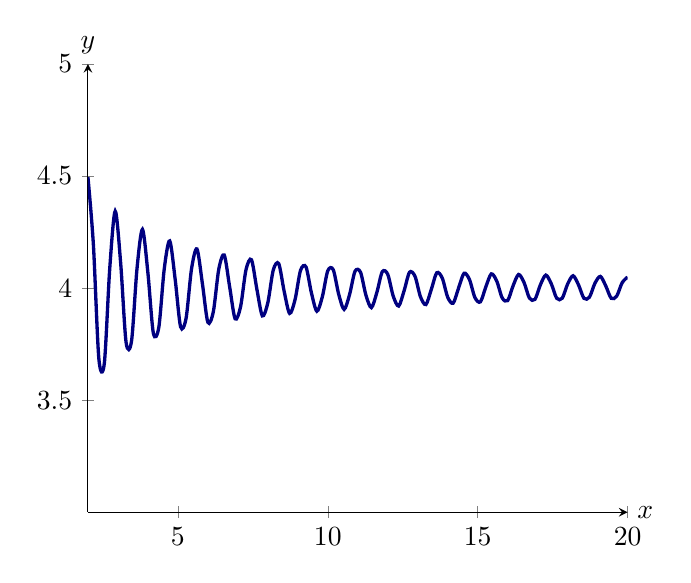
\begin{tikzpicture}
	\begin{axis}[
            domain=2:20,
            ymax=5,
            ymin=3,
            samples=100,
            axis lines =middle, xlabel=$x$, ylabel=$y$,
            every axis y label/.style={at=(current axis.above origin),anchor=south},
            every axis x label/.style={at=(current axis.right of origin),anchor=west}
          ]
	  \addplot [very thick, penColor, smooth] {(1/x) * sin(deg(7*x))+4};
        \end{axis}
\end{tikzpicture}

\end{image}

\begin{explanation}
We can bound our function
\[
\frac{-1+4x}{x} \le \frac{\sin(7x)+4x}{x} \le \frac{1+4x}{x}.
\]
Now write with me
\begin{align*}
\lim_{x\to\infty}\frac{-1+4x}{x} \cdot \frac{1/x}{1/x} &= \lim_{x\to\infty}\frac{-1/x+4}{1}\\
&=4.
\end{align*}
And we also have
\begin{align*}
\lim_{x\to\infty}\frac{1+4x}{x} \cdot \frac{1/x}{1/x} &= \lim_{x\to\infty}\frac{1/x+4}{1}\\
&=4.
\end{align*}
Since 
\[
\lim_{x\to \infty} \frac{-1+4x}{x}  = 4 = \lim_{x\to \infty}\frac{1+4x}{x} 
\] 
we conclude by the Squeeze Theorem,
$\lim_{x\to\infty}\frac{\sin(7x)}{x}+4 = 4$.
\end{explanation}
\end{example}






\begin{definition}\label{def:horiz asymptote}\index{asymptote!horizontal}\index{horizontal asymptote}
If  
\[
\lim_{x\to \infty} f(x) = L \qquad\text{or}\qquad \lim_{x\to -\infty} f(x) = L,
\]
then the line $y=L$ is a \dfn{horizontal asymptote} of $f(x)$.
\end{definition}

\begin{example} 
Give the horizontal asymptotes of
\[
f(x) = \frac{6x-9}{x-1}
\]
\begin{explanation}
From our previous work, we see that $\lim_{x\to \infty} f(x) = 6$, and
upon further inspection, we see that $\lim_{x\to -\infty} f(x) =
6$. Hence the horizontal asymptote of $f(x)$ is the line $y=6$.
\end{explanation}
\end{example}


It is a common misconception that a function cannot cross an
asymptote. As the next example shows, a function can cross a horizontal
asymptote, and in the example this occurs an infinite number of times!

\begin{example}
Give a horizontal asymptote of
\[
	f(x) = \frac{\sin(7x)+4x}{x}.
\]
\begin{explanation}
Again from previous work, we see that $\lim_{x\to \infty} f(x) =
\answer{4}$. Hence $y=\answer{4}$ is a horizontal asymptote of $f(x)$.
\end{explanation}
\end{example}


We conclude with an infinite limit at infinity.

\begin{example}
Compute
\[ \lim_{x\to\infty}\sqrt{x}. \]
\begin{image}
\begin{tikzpicture}
	\begin{axis}[
            domain=0:10,
            ymax=4,
            ymin=-1,
            samples=100,
            axis lines =middle, xlabel=$x$, ylabel=$y$,
            every axis y label/.style={at=(current axis.above origin),anchor=south},
            every axis x label/.style={at=(current axis.right of origin),anchor=west}
          ]
	  \addplot [very thick, penColor, smooth] {x^(1/2)};
        \end{axis}
\end{tikzpicture}
\end{image}

\begin{explanation}
The function $\sqrt{x}$ grows slowly, and seems like it may have a
horizontal asymptote, see the graph above. However, if we consider the
square root as the inverse of the function $f(x) = x^2 , \quad x \geq 0$.

\begin{quote}
  $\sqrt{x} = y$ means that $y^2 = x$ and that $y \geq 0$.
\end{quote}

We see that we may square higher and higher values to obtain
larger outputs.  This means that $\sqrt{x}$ is unbounded, and hence
$\displaystyle \lim_{x\to\infty}\sqrt{x}=\infty$.
\end{explanation}
\end{example}


\end{document}
